\section{Introduction}
\label{sec:intro}


\begin{table}[t]
\resizebox{\columnwidth}{!}{%
\begin{tabular}{@{}ccccc@{}}
\toprule
 &  & \cellcolor[HTML]{FFFFFF}{\color[HTML]{333333} \textbf{\begin{tabular}[c]{@{}c@{}}Training time \\ (hours)\end{tabular}}} & \cellcolor[HTML]{FFFFFF}{\color[HTML]{333333} \textbf{\begin{tabular}[c]{@{}c@{}}Cost\\ (\$)\end{tabular}}} & \cellcolor[HTML]{FFFFFF}{\color[HTML]{333333} \textbf{\begin{tabular}[c]{@{}c@{}}Accuracy\\ (\%)\end{tabular}}} \\ \midrule
\multicolumn{1}{c|}{} & \textit{4 K80 transient} & (1.05, 0.17) & (1.05, 0.02) & (91.23, 1.30) \\
\multicolumn{1}{c|}{} & \cellcolor[HTML]{EFEFEF}{\color[HTML]{000000} \textit{1 K80 on-demand}} & \cellcolor[HTML]{EFEFEF}{\color[HTML]{000000} (3.91, 0.03)} & \cellcolor[HTML]{EFEFEF}{\color[HTML]{000000} (2.83, 0.02)} & \cellcolor[HTML]{EFEFEF}{\color[HTML]{000000} (93.07, 0.002)} \\
\multicolumn{1}{c|}{\multirow{-3}{*}{\textbf{\begin{tabular}[c]{@{}c@{}}Training \\ Setup\end{tabular}}}} & \multicolumn{1}{l}{\textit{4 K80 on-demand}} & (0.99, 0.02) & (2.92, 0.05) & (91.20, 1.01) \\ \midrule
\multicolumn{1}{c|}{} & \textit{r = 0 (21 out of 32)} & (0.98, 0.01) & (1.04, 0.01) & (91.06, 1.43) \\
\multicolumn{1}{c|}{} & \textit{r = 1 (8 out of 32)} & (1.13, 0.12) & (1.07, 0.01) & (91.83, 0.90) \\
\multicolumn{1}{c|}{\multirow{-3}{*}{\textbf{\begin{tabular}[c]{@{}c@{}}Transient\\ revocation \\ scenarios\end{tabular}}}} & \textit{r = 2 (2 out of 32)} & (1.45, 0.50) & (1.10, 0.02) & (90.68, 0.30) \\ \bottomrule
\end{tabular}
}
\caption{\textbf{Benefits of transient distributed training.} On average, training with 4 K80 transient GPU servers achieve 3.72X speedup with 62.9\% monetary savings, compared to running on one K80 on-demand GPU server. In addition, we observe at least 1.2\% accuracy drops compared to single GPU server training. However, the slightly lower accuracy is due to training on stale model parameters in distributed asynchronous training. That is, training with 4 K80 servers, regardless of transient or on-demand, produce models with almost identical accuracies. Here $\textit{r = x (y out of 32)}$ denotes that the revocation of $x$ workers happens in $y$ clusters. 
Performance metrics are represented in a tuple of average and standard deviation throughout the paper, unless otherwise specified.}
\label{intro:tbl:motivation}
\end{table}



%Deep learning has seen rapidly growing popularity in recent years due to model accuracy improvements. As models grow deeper and more complex, training them has become increasingly resource consuming. These models often have a lot of parameters and contain layers such as fully connected or convolutional layers. In order to train deep learning models to reach desired accuracies, one often has to process large amount of data, e.g., TB to PBs~\cite{}. This can be a very time-consuming process. 
%
%In order to train deep learning models efficiently, prior works have focused on tuning hyperparamters, parallelizing training as much as possible, and as well as developing efficient distributed frameworks~\cite{tensorflow,and others} to allow training large amount of data and complex models in much faster fashion. For example, researchers at Facebook has successfully trained a ResNet-50~\cite{} on ImageNet-1k dataset~\cite{} using 32 servers that are equipped with eight NVIDIA P100 GPUs~\cite{}. \tian{data or model parallelism??}
%
%Training deep learning models has evolved from single GPU server~\cite{}, single multi-GPU server~\cite{}, all the way to utilize a cluster of GPU servers. Prior work~\cite{}have shown 
%that it is possible to achieve near linear scalability with a cluster of 32 GPU servers~\cite{}. Driven by the need to perform distributed training continuously, as well as the desire to complete distributed in a fast and cheap manner, it is important to be able to speed up the training process given a predefined monetary budget. 
%
%Often GPU servers can be very costly ranging from XX to YY. \tian{costs for reasonable gpu servers for training DNN.}Recently, major cloud providers start to offer cloud-based GPU servers which make it possible to take advantage of these GPU servers on-demand and speed up the training time. Moreover, cloud providers also offer a much cheaper option of revocable GPU servers that are relatively cheaper (up to XX\%~\cite{}) but can become unavailable with short notice.  As a result, if utilized properly, cloud GPU transient servers can be very beneficial to both improving training speed and reducing training cost. 
%
%To demonstrate the \emph{real-world} benefits of distributed training on transient servers, we launched 32 clusters running with four \texttt{K80} transient GPU servers in google cloud platforms. All clusters use parameter server-based asynchronous training (more detail at Section~\ref{subsec:ddl}). In Figure~\ref{intro:motivation}, we plot the training status for each cluster including the number of revocations, the relative time a GPU server was revoked, and the training performance measured in terms of converged accuracy, time to convergence and the training cost. We observe that 21 out of 32 transient clusters completed training with 0 revocation (last row), and that 13 out of 132 K80 transient servers were revoked during various training stages---the lighter the shade, the earlier the revocation. The key takeaway is that although more than half of the clusters can finish training without revocation, in cases that GPU servers were revoked, training performance (in particular training time) can be negatively impacted.
%
%In Table~\ref{intro:tbl:motivation}, we observe significant improvement of training time and cost reduction using cheaper transient servers, when compared to training on a simple GPU server. The speedup can be up to 3.72X when provided with the initial budget of one single K80 on-demand server. Moreover, distributed training with 4 \texttt{K80} GPU servers also lead to more than 62.9\% saving in training cost with slightly degraded accuracy ($\sim$1.2\%) at convergence time. However, the slightly lower accuracy is due to training on stale model parameters in distributed asynchronous training. That is, training with 4 K80 servers, regardless of transient or on-demand, produce models with almost identical accuracies. 
%%Intuitively, the more initial budget we have, e.g., a more powerful V100 server vs. an older K80 server, the more likely we can improve the training performance. Note that we can achieve very similar convergence accuracy compared to single GPU server training. 
%
%% f = 1 and f = 2 case 
%% (1.13 * 8 + 1.45 * 2) / 10 = 1.194 hr; 3.91 / 1.194 = 3.27X;
%% cost: (1.07 * 8 + 1.1 * 2) / 10 = 1.076 $ ; (2.83 - 1.076) / 2.83 = 62%
%% f = 0 to f=2 
%% 1.45/0.98 = 1.479
%Our empirical analysis reveals three important observations: first distributed training will fail  (happens 3\% of time) when all GPU servers are revoked, or when one GPU server that is responsible for performing checkpoint (master) fails. Second, when some of the GPU servers are revoked(happens 31.25\% of time), the training can continue and finish successfully with an average speedup of 3.27X and cost saving of 62\%. Third, the number of revoked GPU servers has little impact on the training cost and accuracy but causes significant degradation in training time (up to 48\%). This implies that we could mitigate the revocation impact on distributed training performance by increasing the cluster size. We empirically evaluate this hypothesis in Section~\ref{subsec:scaling_out}.
%
%%reduce the total training time and therefore the likelihood of revocations, therefore motivating requesting a cluster as large as possible. \tian{We can plot the saving for losing 1, 2, 3, servers individually.} 
%
%However, much of prior work on distributed training assume access to a cluster of static GPU servers and that these GPU servers are from the data center location. Such assumptions do not hold true when we need to utilize cheap transient GPU servers that could spread across geographically different data center locations. Instead, our system should handle a dynamic transient GPU server market and select the most suitable cluster configuration, so as to achieve convergence accuracy sooner without violating the monetary cost budgets. 
%
%In this paper, we introduce a system, called \sysname, the explores the feasibility and benefits of using cloud transient GPU servers. We first conduct measurement that characterize transient GPU servers’ capabilities and lifetime, and then quantify the training speed improvement with a dynamic cluster configuration. We summarize our contributions as following: 
%
%\begin{itemize}
%\item We empirically evaluate the performance impact of conducting distribute training on transient servers with dynamic availability. We quantify the training speed and accuracy for switching to different cluster configurations. Our measurement results shed lights in designing transient resource management algorithms for distributed training. 
%\item Elastic distributed training with cheap transient servers. Cheaper transient servers can be added without restarting the TensorFlow framework, which by default does not provide. Revoked transient servers can be safely removed without impacting the training process of other servers. 
%\item For each observed performance overheads, we propose alternative designs that could make the distributed training framework more transient-aware and friendly. We implement an approach in \sysname that allows us to dynamically resizing the training cluster with adaptive learning rates, and demonstrate its efficacy in terms of training accuracy and speed. 
%\end{itemize}

Distributed training is an attractive solution to the problem of scaling deep
learning to training larger, more complex, and more accurate models. In short,
distributed training allows models to be trained across a cluster of machines
in a fraction of the time it would take to train on a single server. For
example, researchers at Facebook achieved near linear scalability when training
a ResNet-50 model on the ImageNet-1k dataset using 32 GPU-equipped
servers~\cite{goyal2017accurate}.

Distributed training is especially attractive for companies that want to
leverage cloud-based servers.  All major cloud providers---Google, Microsoft,
and Amazon---offer GPU server options to support deep learning.  However,
existing distributed training frameworks make traditional assumptions about the
lifetime of cloud servers in its cluster. Namely, that once a server is
acquired by the customer it will remain available until \emph{explicitly} released
back to the cloud provider by that customer. In this paper, we refer to such
servers as \emph{on-demand}. While this assumption is reasonable for many
deployments, we argue that it also represents a missed opportunity.   

In this work, we ask the question: what if we use \emph{transient} rather than
\emph{on-demand} servers for distributed training.  Transient servers offer
significantly lower costs than their on-demand equivalents with the added
complication that the cloud provider may \emph{revoke} them at anytime---violating the
availability assumption discussed in the preceding paragraph.  Google,
Microsoft, and Amazon all offer transient servers, so the idea of 
distributed training with transient servers is applicable to all three major
cloud platforms

Consider the following motivating experiment. Using a single on-demand GPU
server on Google Compute Engine, we were able to train a \emph{ResNet-32} model in 3.91 hours
with a total cost of \$2.83 on average (Table~\ref{intro:tbl:motivation}). When we use distributed training with
four on-demand servers---with each machine identical to the single server used 
the in previous runs---we improved the average training time to 0.99 hours
with similar overall cost of \$2.92. Finally, when we use distributed training
with four \emph{transient} servers we retain the improvement in training time,
1.05 hours on average, while significantly reducing the total cost to \$1.05 on
average (Figure~\ref{intro:motivation}). We saw these performance increases even though we made no significant
modifications to the distributed training frameworks and 13 of the 128 transient
servers (affecting 11 out of the 32 clusters) were revoked at some point prior
to the completion of training. We provide a more detailed analysis of this
experiment and the impact of server revocation in Section~\ref{sec:exp}.      

Our goal is to identify the important design considerations needed for
rearchitecting distributed training frameworks to support transient servers.
While the simple experiment above demonstrates the potential of distributed
training with transient servers (e.g., reduced training time and cost) as well
as the challenges (e.g., server revocation and availability), we believe that
transient servers also offer additional opportunities.  For example, price
dynamics make it more attractive to use clusters with machines drawn from
multiple, geographically-diverse, data centers. Such an approach raises
interesting questions about the impact of communication costs and latency on
training performance. Similarly, rather than use a cluster composed of servers 
of the same type,  we might employ heterogeneous clusters composed of machines
with different computational resources and capabilities. Finally, the clusters
themselves need not be static; instead, we might dynamically add or remove
servers to make distributed training more robust to server revocation or to
take advantage of volatile server pricing.   

% Observation version --- risky 
%We conduct the first \emph{large-scale} empirical measurement study that 
%quantifies the training performance of deep learning models using cloud transient servers. 
%In summary, we make the following observations. 
%
%\begin{itemize}
%\item Transient servers exhibit great potential in speeding up distributed training, while also reduce training cost. 
%\item When training with transient servers, it is better to use larger cluster size to mitigate the revocation impact. 
%\item The current distributed training framework is inefficient in handling server revocations. 
%\end{itemize}

We conduct the first \emph{large-scale} empirical measurement study that 
quantifies the training performance of deep learning models using cloud transient servers.  
Through our study, we make the following additional contributions: 
\begin{itemize}
%\item We conduct the first \emph{large-scale} empirical measurement study that quantifies the training performance of deep learning models using cloud transient servers. 
\item We compare the training time and cost of distributed training using transient servers to on-demand servers. We observe up to 7.7X training speedup and up to 62.9\% monetary savings
in one of the distributed training experiment when compared to the single GPU baseline. 
%our empirical analysis identifies the significant performance improvements with speeding up deep learning by almost 8X with more than 60\% monetary savings. 
\item We quantify the revocation impacts of transient servers on training performance and identify the importance of larger cluster sizes and the need to redesign distributed training frameworks. In addition, our observations about model accuracy reveal the opportunities for mitigating revocation impacts if cloud providers were to support \emph{selective} revocation. 
\item We also demonstrate the benefits and limitations of using heterogeneous servers in distributed training. In particular, our findings suggest a number of plausible transient-aware designs for deep learning frameworks, including the ability to train with dynamic cluster sizes, to better exploit these cheap transient servers. 
\end{itemize}


\begin{figure}[t]
\centering
    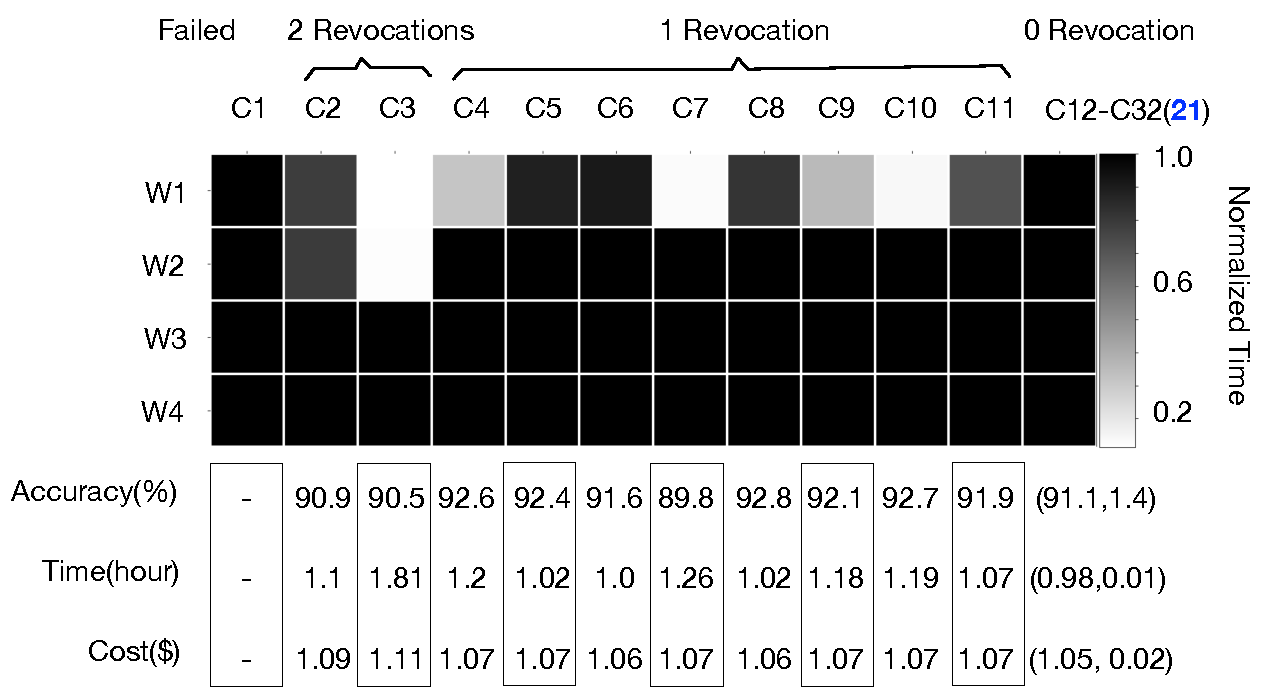
\includegraphics[width=\columnwidth ]{cluster_4_spots_heatmap.pdf}
\caption{\textbf{Quantifying distributed training performance using transient servers.} We launched \emph{32} transient GPU clusters for training ResNet-32 model on Cifar-10 dataset. Each cluster $C_i$ is configured with four \texttt{K80} transient GPU servers($W1$ to $W4$) and one parameter server. We observe that 21 out of 32 transient clusters completed training with 0 revocation, and that 13 out of 128 \texttt{K80} transient servers were revoked during various training stages---the lighter the shade, the earlier the revocation. On average, training with 4 \texttt{K80} transient GPU servers achieve 3.72X speedup and 62.9\% monetary savings, compared to running on one \texttt{K80} on-demand GPU server.}  % 3.91 / 1.05 = 3.72X (time), (2.83-1.05) / 2.83 = 62.9% (cost)
%90\% of the transient servers and 65\% transient servers finish training without revocations, and achieve XX speedup with YY monetary savings compared running on single on-demand GPU server.}
    \label{intro:motivation}
\end{figure}